%\documentclass[letterpaper, 12pt]{report}
\documentclass[letterpaper, 11pt]{article}

%\usepackage{float}
%\floatplacement{figure}{H}

%\author{Brian Bell}
%\date{2-10-2013}
%\title{Humans as Property in the Early West: \\ Contrasting the Origins and Operation of Russian Serfdom with the Peculiar Instituton of Slavery in the United States.}
%\affiliation{2102055378 \\ HST-104 (10162)}


%\usepackage[dvips]{graphicx}
%\usepackage[pdftex]{graphicx}
\usepackage{graphicx}
%\usepackage[dvipdfmx]{graphicx}
\DeclareGraphicsExtensions{.eps,.pdf,.jpg,.png}

%\usepackage[caption=false,labelfont=sf,textfont=sf,captionskip=5pt]{subfig}

%\DeclareGraphicsRule{.pnXg}{eps}{.bb}{}

\usepackage{achicago}
\usepackage{fullpage}
%\usepackage[top=1in, bottom=1in, left= 1 in, right=1in]{geometry}
%\usepackage[top=1.5in, bottom=1.5in, left=1.5in, right=1in]{geometry}
\usepackage{geometry}

%\usepackage{diagbox}

% *** MATH PACKAGES ***
%
%\usepackage{amsmath}
\usepackage[cmex10]{amsmath}
\usepackage{amsfonts}
\usepackage{mathtools}
% A popular package from the American Mathematical Society that provides
% many useful and powerful commands for dealing with mathematics. If using
% it, be sure to load this package with the cmex10 option to ensure that
% only type 1 fonts will utilized at all point sizes. Without this option,
% it is possible that some math symbols, particularly those within
% footnotes, will be rendered in bitmap form which will result in a
% document that can not be IEEE Xplore compliant!
%
% Also, note that the amsmath package sets \interdisplaylinepenalty to 10000
% thus preventing page breaks from occurring within multiline equations. Use:
%\interdisplaylinepenalty=2500
% after loading amsmath to restore such page breaks as IEEEtran.cls normally
% does. amsmath.sty is already installed on most LaTeX systems. The latest
% version and documentation can be obtained at:
% http://www.ctan.org/tex-archive/macros/latex/required/amslatex/math/





% *** SPECIALIZED LIST PACKAGES ***
%
 \usepackage[ruled, boxed]{algorithm2e}
 \usepackage{algorithmic}

%\usepackage{natbib}
%\usepackage[natbib=true, bibstyle=authoryear, citestyle=authoryear-comp]{biblatex}

% for distance between bib items
\usepackage{bibspacing}
\setlength{\bibitemsep}{1.0\baselineskip plus .05\baselineskip minus .05\baselineskip}

%\usepackage[super,sort&compress]{natbib}

\usepackage{layout}

\usepackage{setspace}


\usepackage[nopar]{lipsum} % for dummy text
\usepackage[american]{babel}
\usepackage[babel]{csquotes}
%\usepackage{natbib}
%\usepackage[notes,natbib,isbn=false,backend=biber]{biblatex-chicago}
%\addbibresource{bibfile.bib}

\usepackage{fancyhdr}

%\fancyhf{}
%\fancyhead[C]{\thepage}
%\pagestyle{fancy}

% redefine the plain pagestyle
%\fancypagestyle{plain}{%
%\fancyhf{} % clear all header and footer fields
%\fancyhead[C]{\thepage} % except the center
%}

%\usepackage{chicago}
%\usepackage{fancyhdr}
\pagestyle{fancy}
%\fancyhead[R]{Humans as Property in the Early West - \thepage}
\fancyhead[R]{\thepage}
\fancyfoot{}
\renewcommand{\headrulewidth}{0pt}
\renewcommand{\footrulewidth}{0pt}


%\newcommand{\HRule}{\rule{\linewidth}{0.25mm}}
\newcommand{\HRule}{\rule{\linewidth}{0mm}}

\doublespacing
%\setlength{\parindent}{0pt}

% 36pt == 0.5in


\setlength{\voffset}{0in}
\setlength{\hoffset}{0in}

\setlength{\marginparpush}{0in}
\setlength{\footskip}{0in}

\setlength{\marginparsep}{0in}
\setlength{\marginparwidth}{0in}

\setlength{\textheight}{578pt}
\setlength{\textwidth}{434pt}



%\setlength{\oddsidemargin}{0.5in}

\setlength{\topmargin}{0in}
\setlength{\headheight}{0in}
\setlength{\headsep}{0.5in}

\setlength{\footnotesep}{24pt}
%\setlength{\skip\footins}{0pt}

%\setlength{\parindent}{4em}

%\setlength\bibitemsep{1.5\itemsep}
%\setlength{\bibitemsep}{1.5in}


\begin{document}%\layout
\begin{titlepage}
\begin{center}

\HRule

\textbf{\Huge IMDB Sentiment Analysis} \\
\bigskip\bigskip\bigskip\bigskip\bigskip\bigskip\bigskip\bigskip\bigskip\bigskip\bigskip
{Group 11: }\\
{Marc Andre Rousseau (fake number 12345678 to be updated)}\\
{Robin Luo (260851506)}\\
{Bide Xu (260711367)}\\
\bigskip\bigskip\bigskip\bigskip\bigskip\bigskip\bigskip\bigskip\bigskip\bigskip\bigskip
{Course Number: COMP 551}\\
{Course Name: Applied Machine Learning}\\
{\today}

\end{center}
\end{titlepage} 

\clearpage
\setcounter{page}{2}
%\autocite{citekey} just use footnotes!

\singlespacing

\begin{abstract}
This project was purposed to assess the performance 

\end{abstract}

\section*{Introduction}

IMDB  is frequently ...



\section*{Related work}



\section*{Dataset and Setup}

Let us test some math formula, ``$X^{3}$''

\section*{Proposed approach}



\section*{Results}

All our experiment results are stored as .json file, which will be submitted with the source codes and other documents. The performance ... are summerized in Table \ref{tbl:table_fp}, and discussed as following:

\subsection*{1}

Let us test some figure here:

\begin{figure}[!ht]
  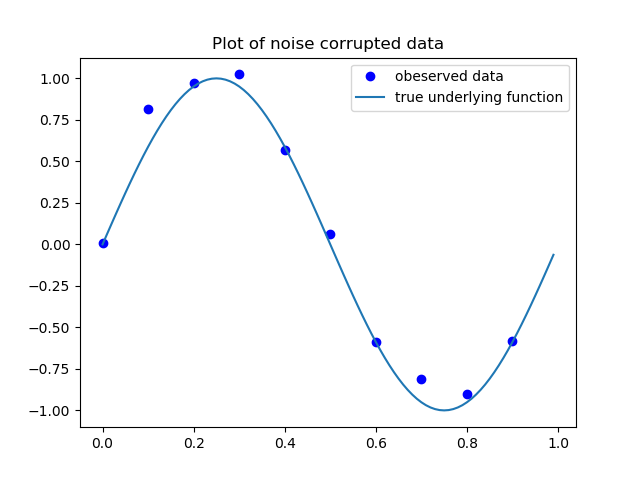
\includegraphics[width=\linewidth]{fig/figure_3.png}
  \caption{run time, accuracy performance comparsion ...}
  \label{fig:cf_vs_gd}
\end{figure}


\subsection*{2}

Let us test some table here 


\begin{table}[]
\centering
\begin{tabular}{|l|l|l|l|l|l|}
\hline
\textbf{Feature(s) w.r.t Performance}                                                                                                                                     & \textbf{\begin{tabular}[c]{@{}l@{}}MSE of \\ Training \\ Data\end{tabular}} & \textbf{\begin{tabular}[c]{@{}l@{}}MSE of \\ Validation \\ Data\end{tabular}} & \textbf{\begin{tabular}[c]{@{}l@{}}MSE of \\ Testing \\ Data\end{tabular}} & \textbf{\begin{tabular}[c]{@{}l@{}}run time \\ (in S)\end{tabular}} & \textbf{\begin{tabular}[c]{@{}l@{}}pre-run time \\ (in S) \\ time for \\ computing \\ text/numeric \\ features\\ and generate \\ related matrix\end{tabular}} \\ \hline
\textbf{\begin{tabular}[c]{@{}l@{}}Basic Model \\ (3 numeric  features)\end{tabular}}                                                                                     & 1.084683                                                                    & 1.020326                                                                      & 1.297531                                                                   & 0.027982                                                            & 3.207755                                                                                                                                                      \\ \hline
\textbf{Model With:}                                                                                                                                                      &                                                                             &                                                                               &                                                                            &                                                                     &                                                                                                                                                               \\ \hline
\textbf{“60 high frequency  words”}                                                                                                                                       & 1.059316                                                                    & 0.969286                                                                      & 1.298629                                                                   & 0.026985                                                            & 88.564367                                                                                                                                                     \\ \hline
                                                                                                                                                    \\ \hline
\end{tabular}
\caption{Performance Evaluation For Varies Implemented Features and Their Combinations}
\label{tbl:table_fp}
\end{table}


\section*{Discussion and Conclusion}

This project indicated better results of ...

\section*{Contribution Statement}

All members brainstormed for .
\begin{itemize}
	\item Marc Andre Rousseau:
	\item Robin Luo: 
    \item Bide Xu: 
\end{itemize}

All participated in whole progress and learnt through this project.


\nocite{*}

\bibliographystyle{achicago}



\begingroup

    %\setlength{\bibsep}{10pt}

    \setstretch{1}
    \bibliography{bibfile}


\endgroup
%\renewcommand{\baselinestretch}{2.1}
\renewcommand{\thepage}{}

%\bibliography{bibfile}

%\setlength{\bibitemsep}{1.5itemsep}
%\setlength{\bibnamesep}{1.5itemsep}
%\setlength{\bibinitsep}{1.5itemsep}



%\pagestyle{fancy}
%\fancyhead[R]{\thebibliography}
%\fancyfoot{}
%\renewcommand{\headrulewidth}{0pt}
%\renewcommand{\footrulewidth}{0pt}


%\begin{figure}
%  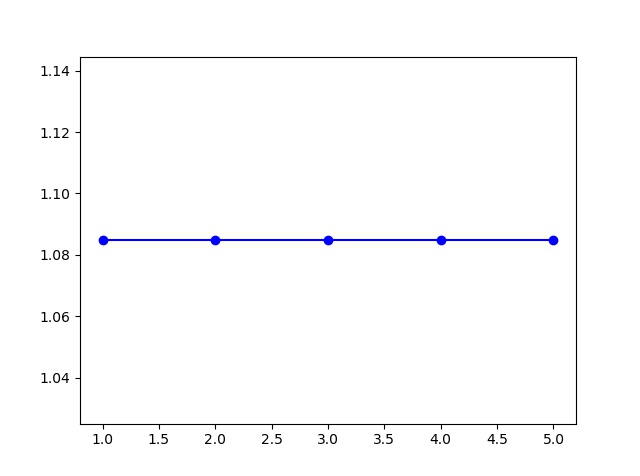
\includegraphics[width=\linewidth]{fig/pic1.jpg}
%  \caption{Relationship among }
%  \label{fig:relation1}
%\end{figure}




\end{document} 